
\documentclass[a4 paper,12pt]{article}
\usepackage[inner=2.0cm,outer=2.0cm,top=2.5cm,bottom=2.5cm]{geometry}
\usepackage{setspace}
\usepackage{appendix}
\usepackage[rgb]{xcolor}
\usepackage{tabu}
\usepackage{multirow}
\usepackage{longtable}
\usepackage{graphicx}
\usepackage{verbatim}
\usepackage{longtable}
\usepackage{subcaption}
\usepackage{fancyhdr}
\usepackage[colorlinks=true, urlcolor=blue, linkcolor=blue, citecolor=blue]{hyperref}
\usepackage{booktabs}
\usepackage{amsmath,amsfonts,amsthm,amssymb}
\usepackage{setspace}
\usepackage{fancyhdr}
\usepackage{lastpage}
\usepackage{tikz}
\usepackage{listings}
%\lstset{
	%	commentstyle=\color{red!50!green!50!blue!50},%代码块背景色为浅灰色
	%	rulesepcolor= \color{gray}, %代码块边框颜色
	%	breaklines=true,  %代码过长则换行
	%	numbers=left, %行号在左侧显示
	%	numberstyle= \small,%行号字体
	%	keywordstyle= \color{blue},%关键字颜色
	%	frame=shadowbox,%用方框框住代码块
	%	basicstyle=\ttfamily
	%}
\definecolor{dkgreen}{rgb}{0,0.6,0}
\definecolor{mauve}{rgb}{0.9,0.1,0.4}
\definecolor{ash}{rgb}{0.8,0.8,0.8}
\lstset{ 
	language=Octave,                % the language of the code
	basicstyle=\ttfamily,           % the size of the fonts that are used for the code
	numbers=left,                   % where to put the line-numbers
	numberstyle=\small\color{gray},  % the style that is used for the line-numbers
	stepnumber=2,                   % the step between two line-numbers. If it's 1, each line
	% will be numbered
	numbersep=5pt,                  % how far the line-numbers are from the code
	backgroundcolor=\color{ash},      % choose the background color. You must add \usepackage{color}
	rulesepcolor= \color{gray}, %代码块边框颜色
	showspaces=false,               % show spaces adding particular underscores
	showstringspaces=false,         % underline spaces within strings
	showtabs=false,                 % show tabs within strings adding particular underscores
	frame=single,                   % adds a frame around the code
	rulecolor=\color{black},        % if not set, the frame-color may be changed on line-breaks within not-black text (e.g. commens (green here))
	tabsize=2,                      % sets default tabsize to 2 spaces
	captionpos=b,                   % sets the caption-position to bottom
	breaklines=true,                % sets automatic line breaking
	breakatwhitespace=false,        % sets if automatic breaks should only happen at whitespace
	title=\lstname,                   % show the filename of files included with \lstinputlisting;
	% also try caption instead of title
	frame=shadowbox,%用方框框住代码块
	keywordstyle=\color{blue},          % keyword style
	commentstyle=\color{dkgreen},       % comment style
	stringstyle=\color{mauve},         % string literal style
	escapeinside={\%*}{*)},            % if you want to add LaTeX within your code
	morekeywords={*,...}               % if you want to add more keywords to the set
}
\usetikzlibrary{positioning, arrows.meta}
\usepackage{extramarks}
\usepackage{ctex,amsmath,amsfonts,amssymb,bm,hyperref,graphicx}
\usepackage{chngpage}
\usepackage{soul,color}
\usepackage{graphicx,float,wrapfig}
\newcommand{\homework}[3]{
	\pagestyle{myheadings}
	\thispagestyle{plain}
	\newpage
	\setcounter{page}{1}
	\noindent
	\begin{center}
		\framebox{
			\vbox{\vspace{2mm}
				\hbox to 6.28in { {\bf 现代电子电路基础及实验报告 \hfill} {\hfill {\rm #2} {\rm #3}} }
				\vspace{4mm}
				\hbox to 6.28in { {\Large \hfill #1  \hfill} }
				\vspace{3mm}}
		}
	\end{center}
	\vspace*{4mm}
}
\newcommand\numberthis{\addtocounter{equation}{1}\tag{\theequation}}

\begin{document}
	\homework{TTL与非门参数测量}{1900011413}{吴熙楠}
	
	\section{实验目的}
	(1)熟悉逻辑函数的建立和化简方法;
	\par (2) 掌握组合逻辑电路的设计和测试方法。
	\section{实验器材}
	直流稳压电源、示波器、信号发生器、万用表、面包板 、TTL芯片。
	\section{实验原理}
    \noindent
\textbf{3.1组合逻辑电路}
\par 组合逻辑电路的特点是任一时刻($t_{i}$)的稳态输出仅决定于同一时刻($t_{i}$)的输入状态,而与前一时刻($t_{i-1}$)的输入状态无关。一般的设计步骤如下:(1)根据逻辑功能的要求,设定逻辑函数的输入变量和输出变量,然后按逻辑功能列
出真值表;(2)由真值表写出逻辑表达式,并进行化简;(3)按表达式画出逻辑电路图;(4)验计设计方案。\\
\noindent
\textbf{3.2半加器}
\par 半加器的功能是完成两个一位二进制数($A_{n}、B_{n}$)的加法运算,要求输出和数($S_{n}$)及
进位数($C_{n}$)。半加器的真值表如下所示:
	\begin{figure}[H]
		\centering
		\hspace{2em}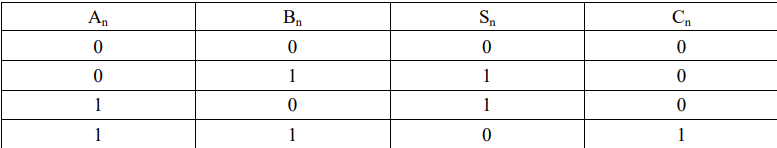
\includegraphics[width=.75\linewidth]{pic/1.png}
		\caption{半加器的真值表
		}
	\end{figure}
\par 用异或门和与门组成的半加器电路如下:
	\begin{figure}[H]
		\centering
		\hspace{2em}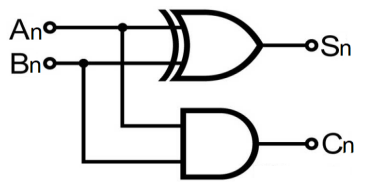
\includegraphics[width=.3\linewidth]{pic/2.png}
		\caption{异或门及与门组成半加器
		}
	\end{figure}
	\section{实验内容(半加器)}
    \noindent
	\begin{figure}[H]
		\centering
		\hspace{2em}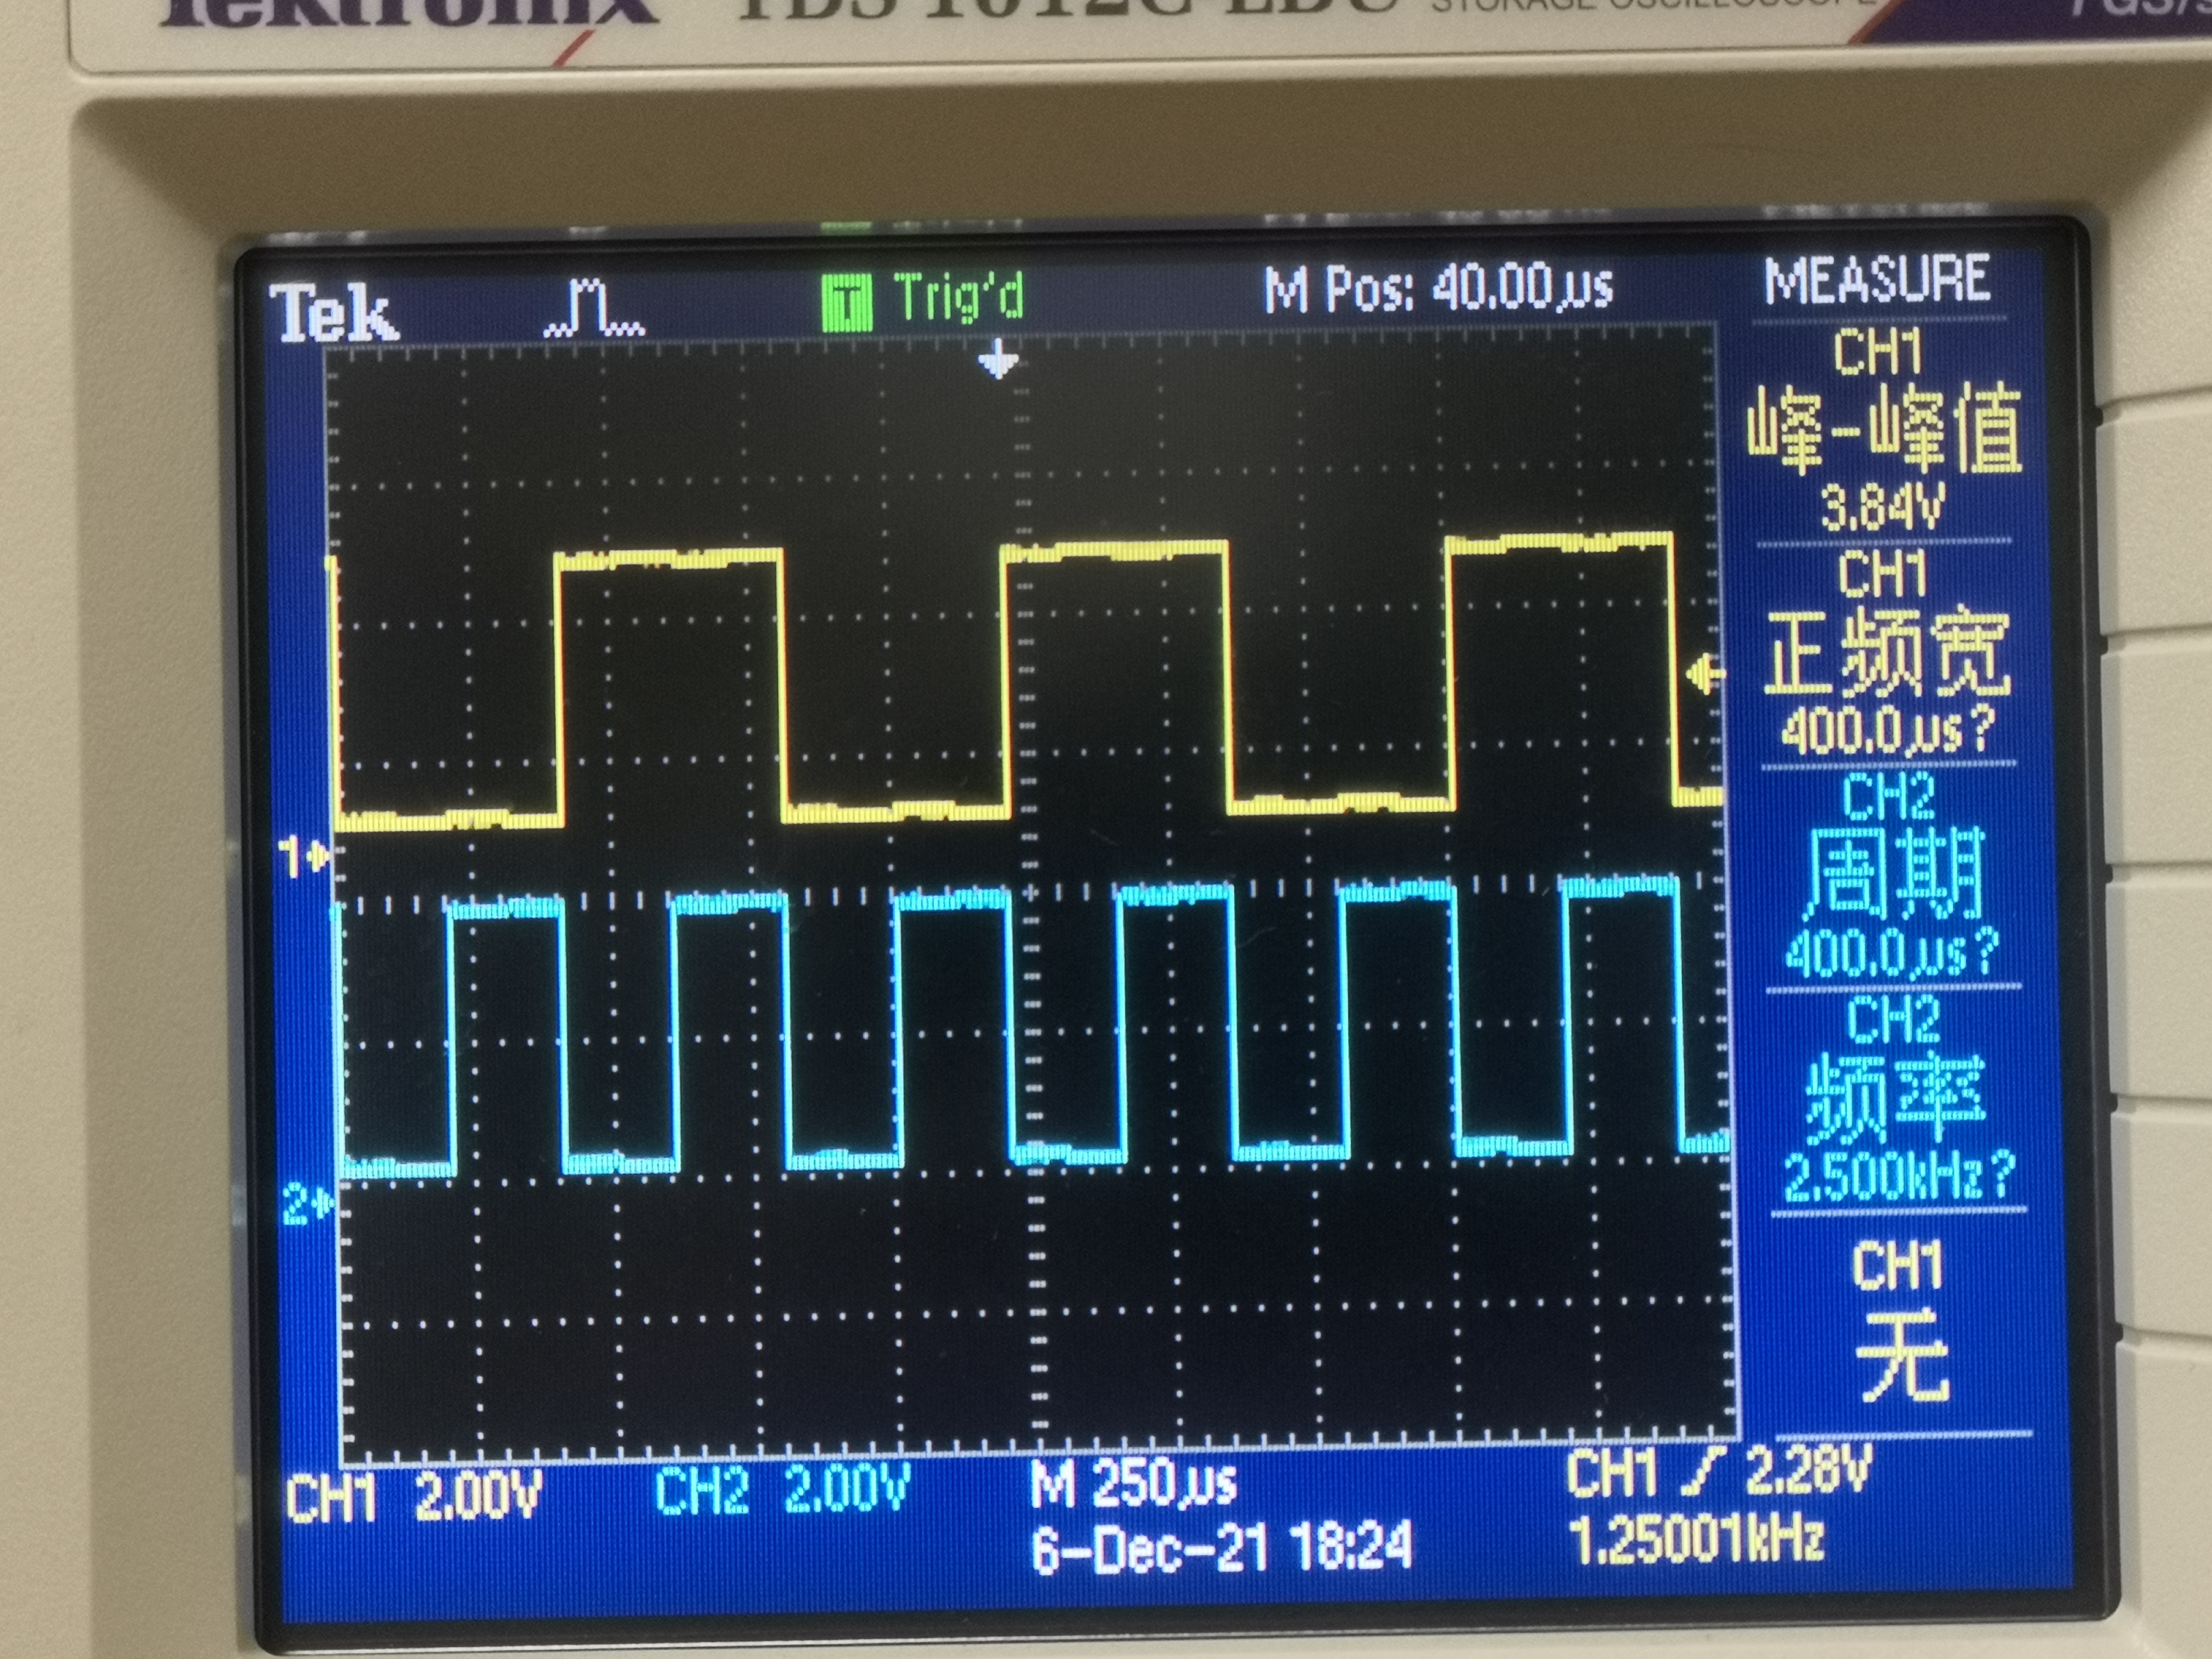
\includegraphics[width=.4\linewidth]{pic/1.jpg}
		\caption{半加器A,B端的输入信号
		}
	\end{figure}
    \par 其中B端输入信号周期为A端输入信号的一半。
	\begin{figure}[H]
		\centering
		\hspace{2em}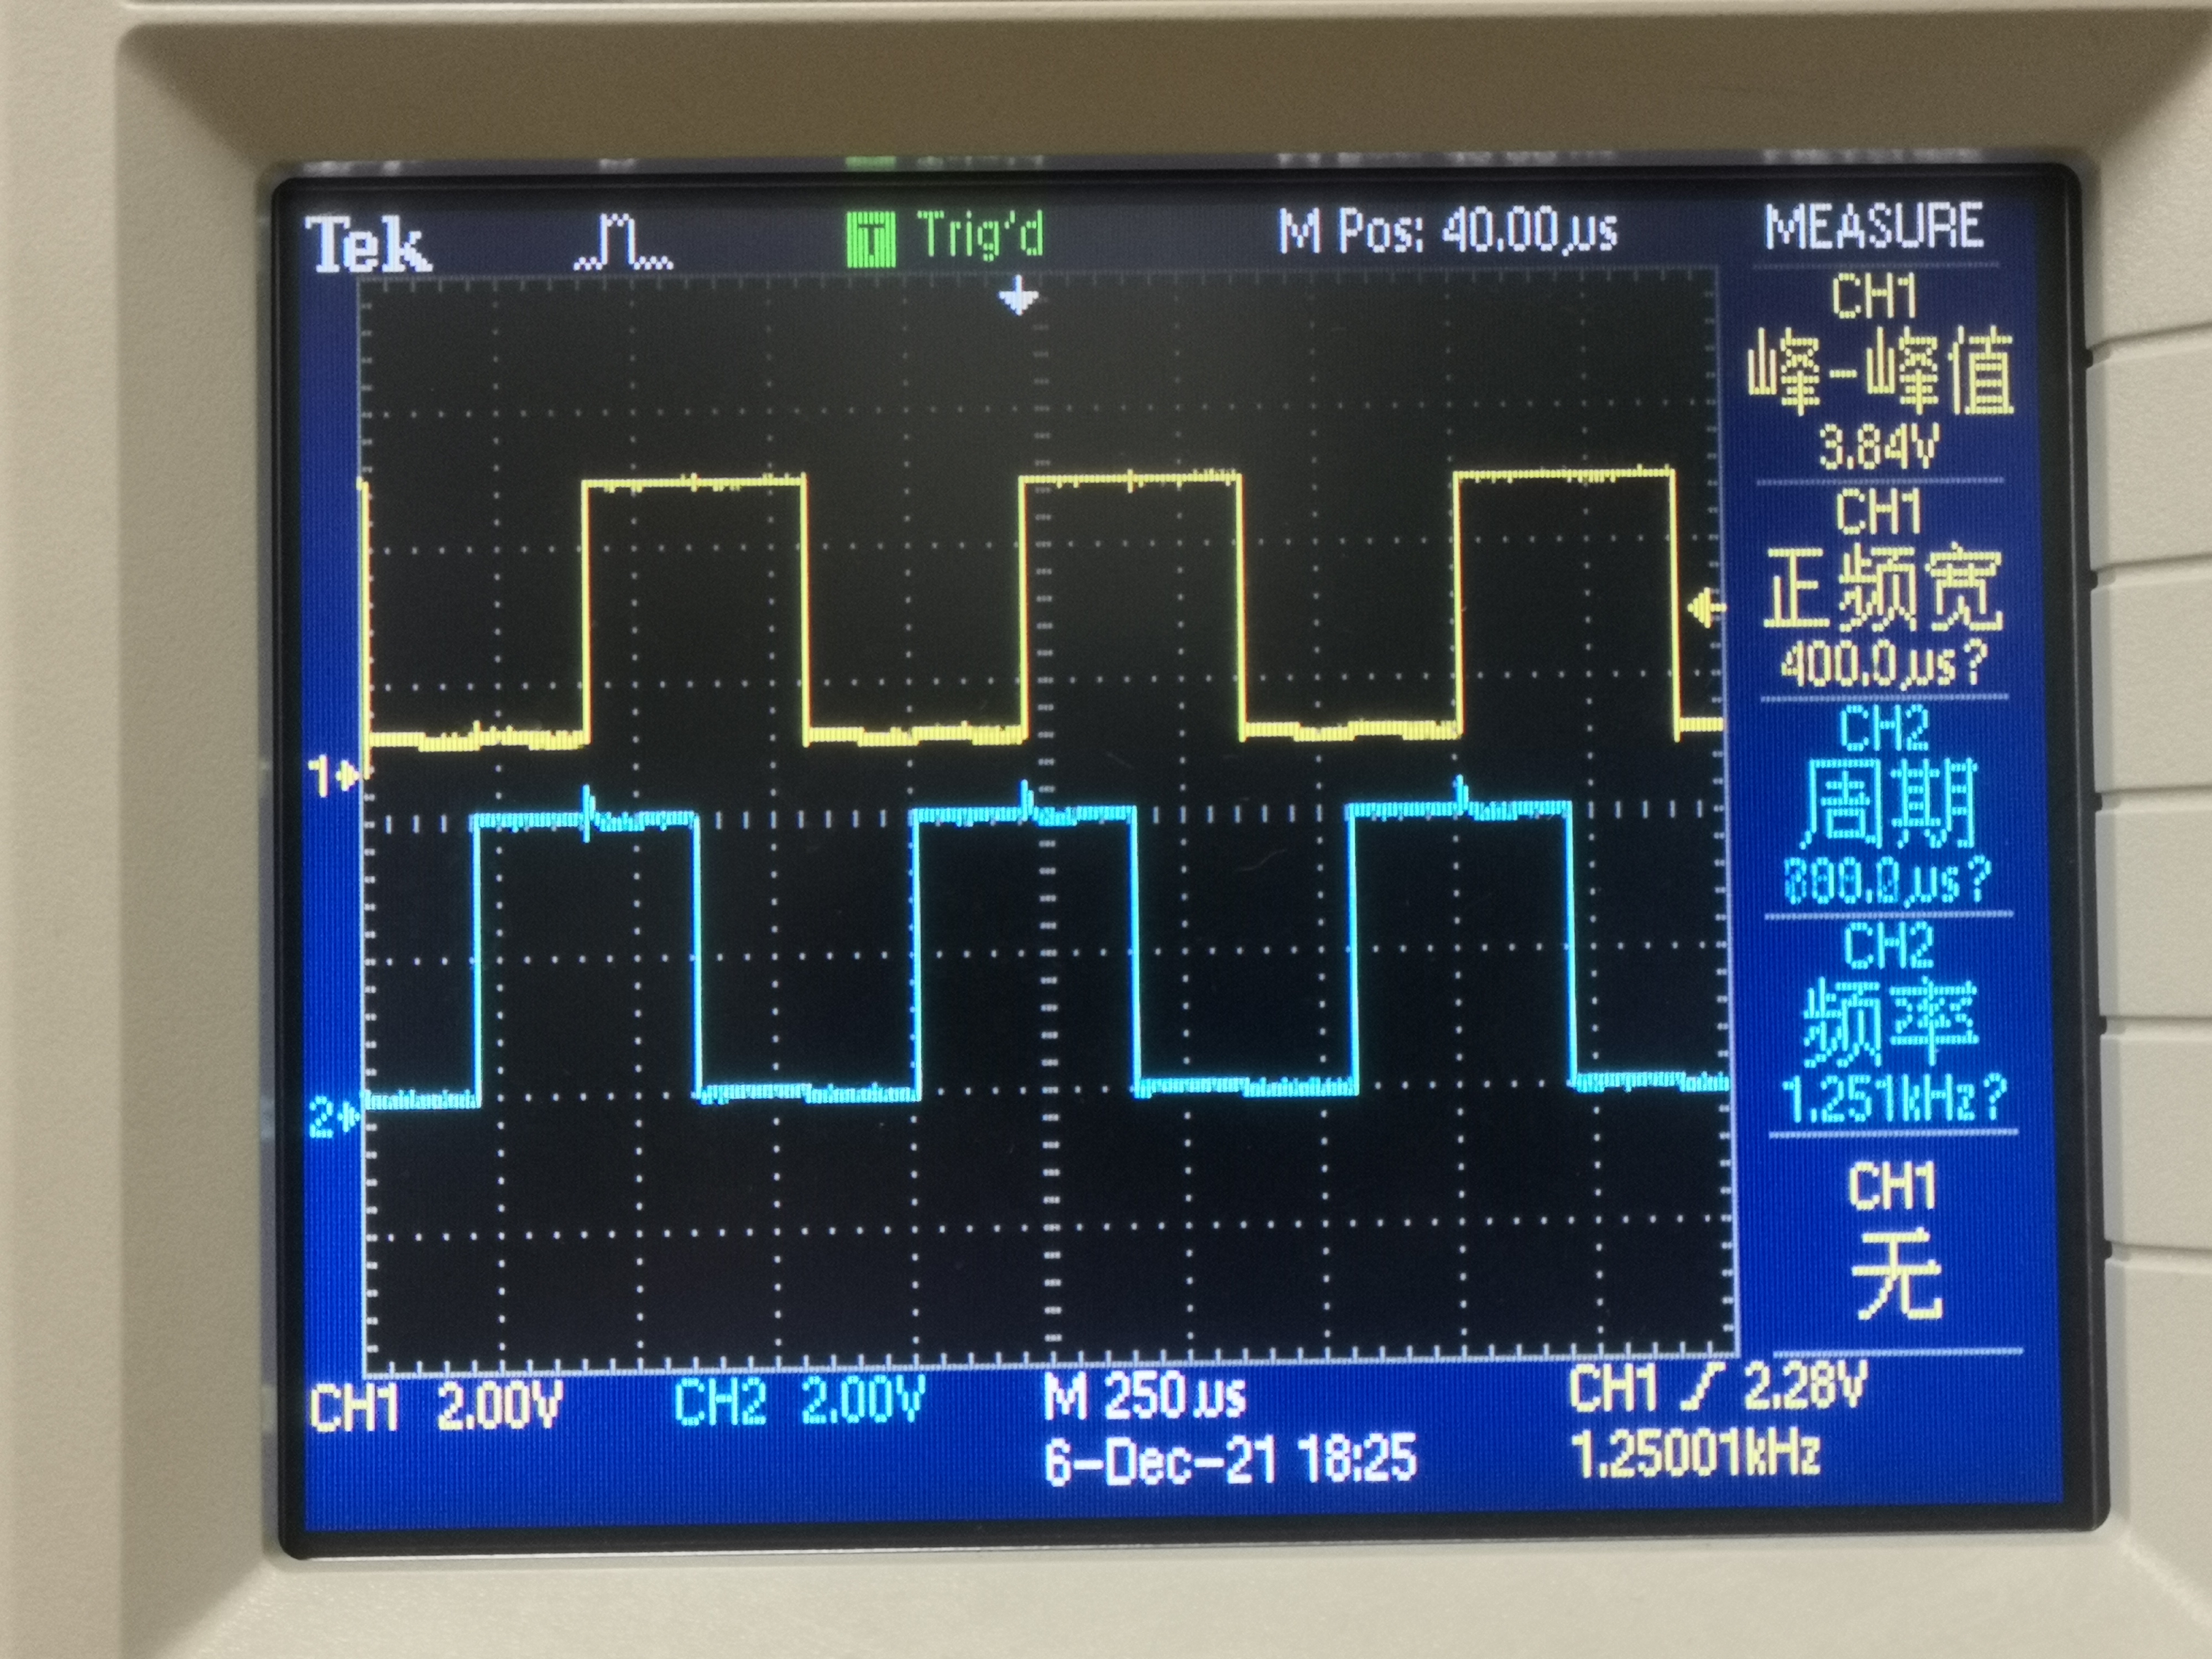
\includegraphics[width=.4\linewidth]{pic/2.jpg}
		\caption{半加器B端的输入信号与和信号
		}
	\end{figure}
    \par 由图中可以看出在A,B信号均为高电平或低电平时候和信号为低电平,一高一低电平时和信号为高电平,满足半加器的逻辑关系。
    \begin{figure}[H]
    		\centering
    		\hspace{2em}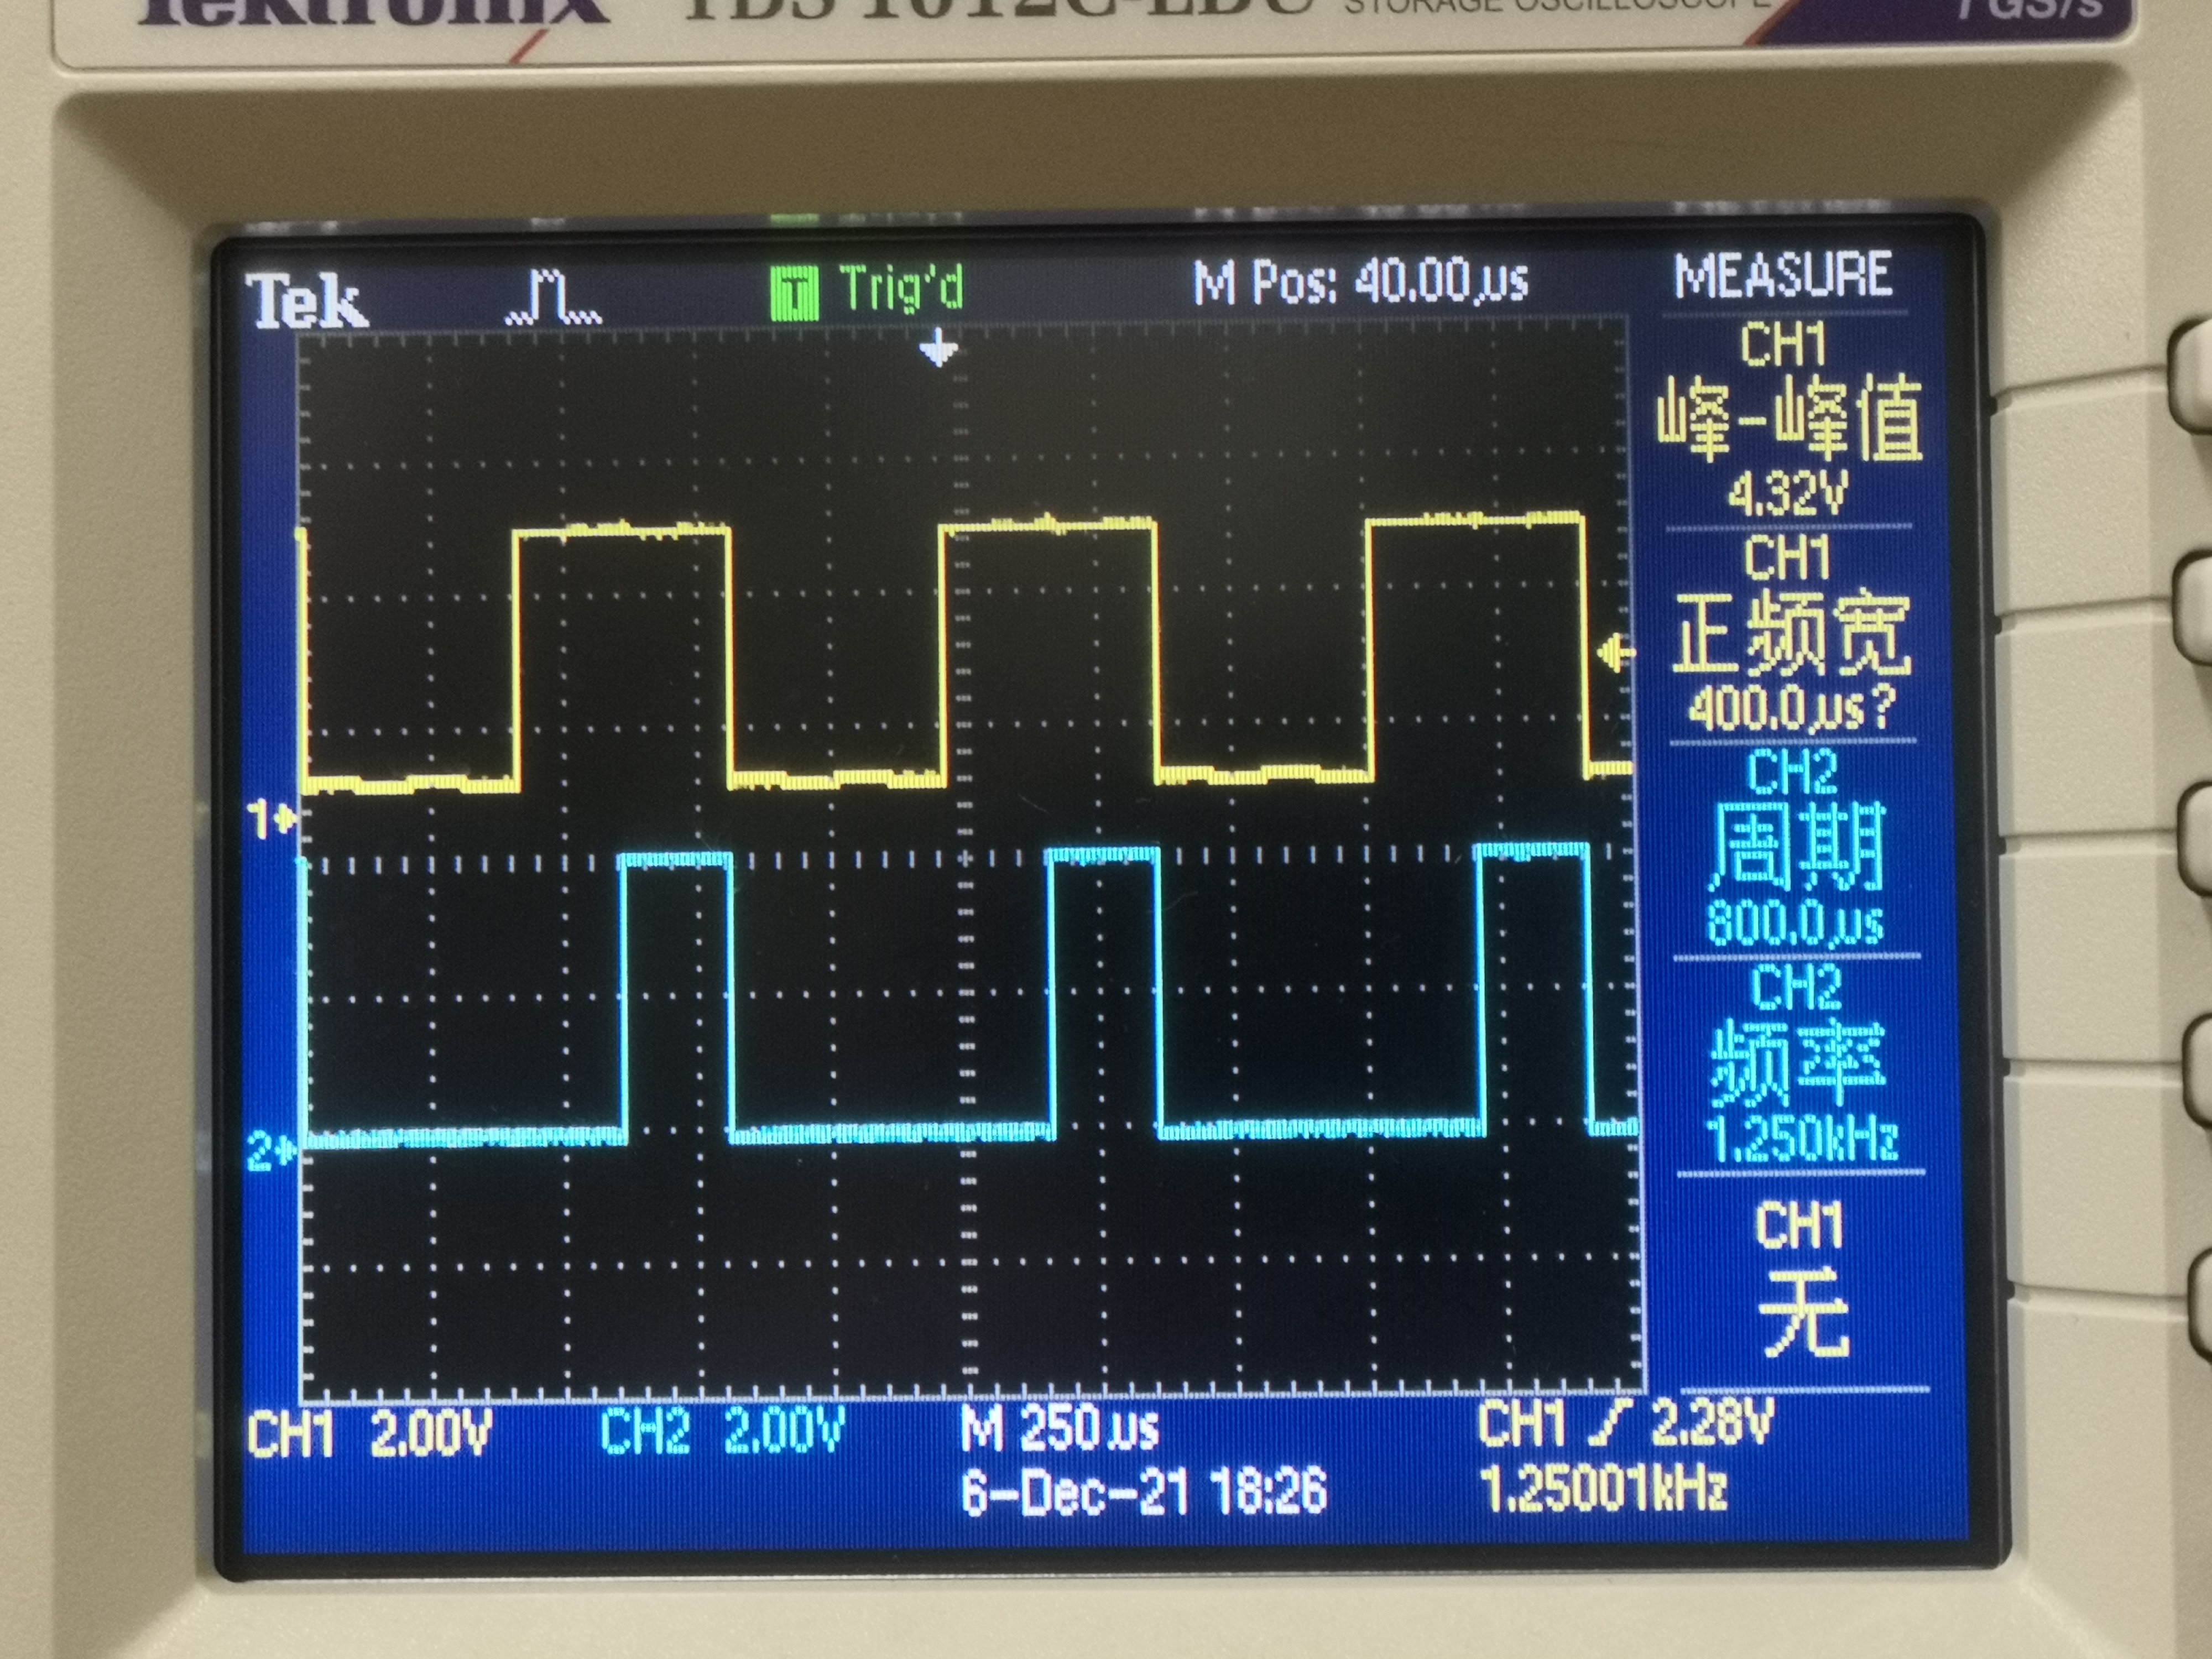
\includegraphics[width=.4\linewidth]{pic/3.jpg}
    		\caption{半加器B端的输入信号与进位信号
    		}
    	\end{figure}
        \par 由图中可以看出,当A,B两端电平均为高电平时进位信号为高电平,表示进位信息,满足其加法的逻辑关系。
	\section{思考题}
	\noindent
	\textbf{1.用二输入与非门实现“四中取三”表决逻辑功能。要求:设定输入输出变量,列出真值表,写出逻辑表达式。}
    \par 我们用A,B,C,D表示输入信号,E表示输出信号
        \begin{figure}[H]
        		\centering
        		\hspace{2em}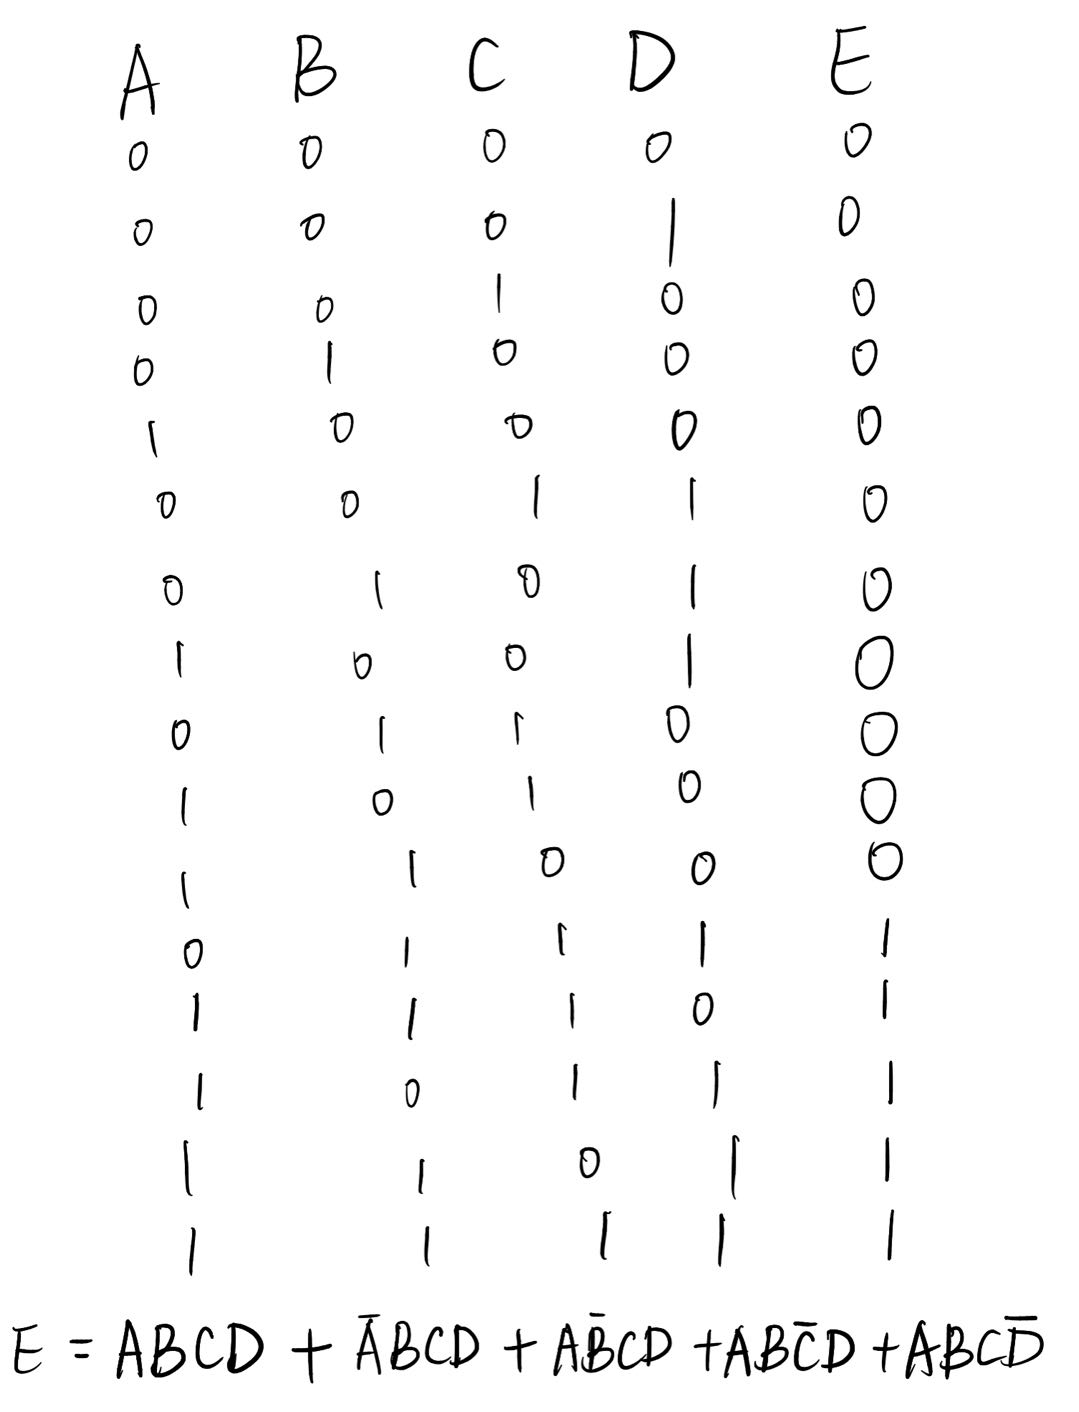
\includegraphics[width=.6\linewidth]{pic/4.jpg}
        		\caption{与非门四中取三表决逻辑关系真值表与表达式
        		}
        	\end{figure}
                \begin{figure}[H]
                		\centering
                		\hspace{2em}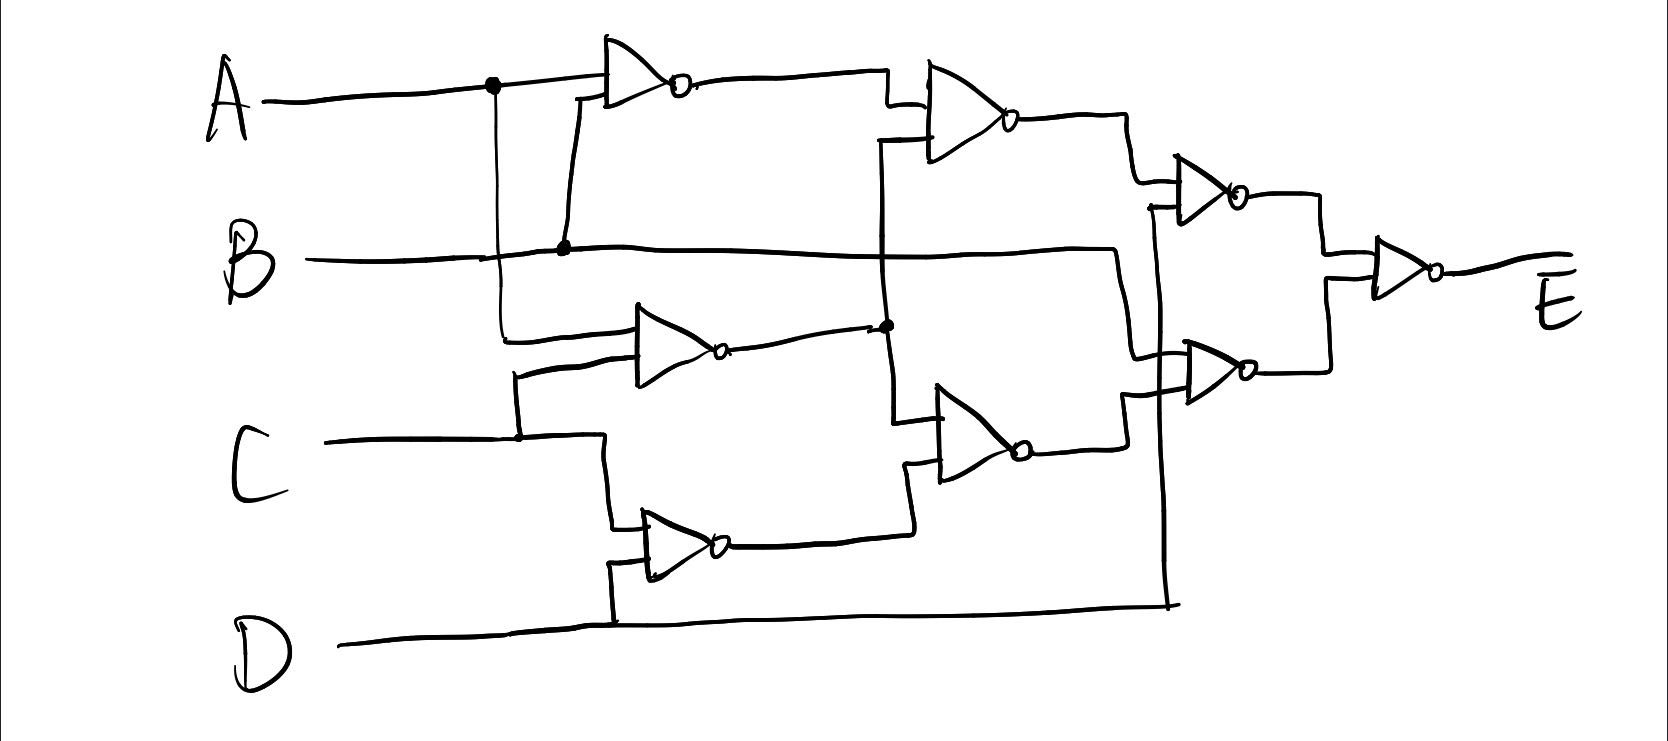
\includegraphics[width=.6\linewidth]{pic/5.jpg}
                		\caption{与非门四中取三表决逻辑电路
                		}
                	\end{figure}
\end{document} 
